\documentclass[aspectratio=169,11pt]{beamer}
\usepackage{teaching_slides}


\title[L8b - Instrumental Variables II]{ Econometrics I}
\subtitle{Lecture 7: Instrumental Variables II --- weak instruments, LATE, judges, shift-share}
\author{Chris Conlon \\NYU Stern}
\date{Fall 2026}

%\usepackage[italic]{mathastext}



%\usepackage{caption,subcaption}
%\usepackage{booktabs}
%\usepackage[flushleft]{threeparttable}


\usepackage{tikz}
\usepackage{pgfplots}
\pgfplotsset{compat=1.7}
\usetikzlibrary{shapes,decorations,arrows,snakes, patterns, angles, quotes, calc,arrows.meta,fit,positioning}
\tikzset{
    -Latex,auto,node distance =1 cm and 1 cm,semithick,
    state/.style ={ellipse, draw, minimum width = 0.7 cm},
    point/.style = {circle, draw, inner sep=0.04cm,fill,node contents={}},
    bidirected/.style={Latex-Latex,dashed},
    el/.style = {inner sep=2pt, align=left, sloped}
}



% Fall 2026: the weak-instrument and overidentification frames were carried over from the
% original IV deck; LATE, judge, and shift-share sections are new. Figures/tables from iv2_sims.R.
% Readings: Hansen Ch. 12; Goff Ch. 4; Mixtape Ch. 7. Workbook: inclass_session7.Rmd

\begin{document}

\maketitle


\begin{frame}{Where we are}
\begin{itemize}
	\item Session 6: why OLS fails under endogeneity, and how an instrument fixes it when everyone has the
	same $\beta$.
	\medskip
	\item Today, three things applied work cannot do without:
	\begin{enumerate}
		\item \alert{Checking the assumptions}, and what happens when the instrument is \alert{weak} --- including
		what changed in the advice since 2020.
		\item What IV estimates when effects \alert{differ across people}: the local average treatment effect,
		and who the compliers are.
		\item The two designs behind most credible IV papers of the last fifteen years: \alert{judges and examiners},
		and \alert{shift-share} exposure.
	\end{enumerate}
	\medskip
	\item Simulations with known answers throughout; Assignment 4 uses the last two designs.
\end{itemize}
\end{frame}

\section{Checking the assumptions; weak instruments}

\begin{frame}{Checking The IV Assumptions I}
\begin{itemize}
\item The two major assumptions:
\begin{enumerate}
	\item Relevance: $Cov(X,Z)\ne 0$, or that $\E\left[{\bf z}_i {\bf x}_i' \right]$ has full rank

	\item Exogeneity: All instruments must be uncorrelated with $\varepsilon$
\end{enumerate}
\smallskip
\item First, let's talk about the relevance assumption.
	\item It's easy to check that the sample analog to $Cov(X,Z)\ne 0$, or the analogous
	matrix condition.
	 \item The more practically relevant concern is that the covariance will be \emph{close}
	 to zero. This is called {\bf weak instruments}.
	 \item How do we test and deal with weak instruments in practice?

\end{itemize}
\end{frame}


\begin{frame}{Weak Instruments I}
\begin{itemize}
	\item In finite samples there's a possibility that the sample covariance
	\begin{align*}
	\sum\limits_{i=1}^N(x_i-\bar{x})(z_i-\bar{z})
	\end{align*}
	is close to zero, especially if the true covariance is relatively small.
	\medskip
	\item Dividing by zero is \emph{bad}.
	\medskip
	\item Note we don't have the same problem in OLS as long as we have variation in the regressors.

\end{itemize}
\end{frame}



\begin{frame}{Weak Instruments II}
\begin{itemize}
\item There is \textbf{big} problem with IV estimation: 2SLS performs \textbf{terribly} in small samples
\medskip
	\item Intuition: Instrumental variables relies on $Corr(X,Z)\ne 0$
		\begin{itemize}
			\item If $Cov(X,Z)=0$ then IV estimator is infinite!
		\end{itemize}
\medskip
	\item In practice, very rarely will $Cov(X,Z)=0$ in data (just randomness)
		\begin{itemize}
			\item Hence, IV will usually ``work" with any choice of $X$ and $Z$
			\item Realistically, sometimes  $Cov(X,Z)$ is small if $Z$ only explains a small portion of $X$
		\end{itemize}
\medskip
	\item If $Cov(X,Z)$ is small we say that $Z$ is a weak instrument

\end{itemize}
\end{frame}



\begin{frame}{Weak Instruments and Small Sample Bias}

Suppose that $Z$ is \emph{a bad instrument} in that $Cov(Z,\varepsilon)$ are correlated

\begin{itemize}
	\item Similar to OVB
		\begin{align*}
			\hat\beta_1^{IV}  \to \beta_1 + \frac{Cov(Z,\varepsilon)}{Cov(Z,X)}\times\frac{\sigma_\varepsilon}{\sigma_X}
		\end{align*}
	\item Compare to OLS case (biased because of OVB):
		\begin{align*}
			\hat\beta_1^{OLS} \to \beta_1 + Cov(X,\varepsilon)\times\frac{\sigma_\varepsilon}{\sigma_X}
		\end{align*}

	\item Which estimator is better here?
		\begin{itemize}
			\item IV's advantage is $Corr(Z,\varepsilon)$ should be smaller than $Corr(X,\varepsilon)$
			\item But if instrument is weak $Corr(Z,X)\approx 0$, then bias blows up even if $Corr(Z,\varepsilon)$ small
		\end{itemize}
\medskip
	\item Danger of weak instruments:
		\begin{itemize}
			\item Very small bias in $Z$ can be greatly magnified if instruments are weak
			\item Amplified bias may have different sign than OLS
		\end{itemize}
\end{itemize}
\end{frame}

\begin{frame}{Weak Instruments and Inference}

To do inference we rely on the CLT:
\begin{align*}
	\hat\beta^{IV} \sim \mathcal{N}\left(\beta, Var\left(\hat\beta^{IV}\right)\right)
\end{align*}

\begin{itemize}
	\item First issue: the Normal Approximation fails unless $N$ is huge! (the CLT does not work well)
		\begin{itemize}
			\item Intuition: $\hat\beta^{IV} = Cov(Y,Z)/Cov(X,Z)$.
			\item If $Cov(X,Z)\approx 0$ then small changes in estimated covariance can have huge effects on estimated coefficients
		\end{itemize}
\medskip
	\item Second issue: even if the normal approximation works the variance explodes!
		\begin{itemize}
			\item Intuition from homoscedastic case: $Var(\hat\beta^{IV})) = \sigma^2/(N\sigma^2_XR^2_{XZ})$
			\item If the $R^2$ of $X$ on $Z$ is very small, then variance is very large
		\end{itemize}
\end{itemize}

\end{frame}

\begin{frame}{How To Deal With Weak Instruments?}

What are we to do if instruments are weak?

\begin{itemize}
		\item Easiest: get more instruments or better instruments
\medskip
		\item Harder: adjust how to do inference
			\begin{itemize}
				\item Turns out that if instruments are weak, asymptotic distribution of $\hat\beta$ will be the \emph{ratio} of two \emph{correlated} normal random variables
				\item We will not pursue this (uses LIML)
			\end{itemize}
\medskip
		\item The good news: We can test $Cov(X,Z)$ by regressing $x_i=\pi_0 + \pi_1 Z_i + \eta_i$
			\begin{itemize}
				\item Since $Z$ and $X$ are data, we can just see if $\hat{\pi}_1$ is far from zero
			\end{itemize}
\medskip
\item \textbf{Rule of Thumb:} Only use instrument if t-stat of null hypothesis that $\pi_1=0$ is $\geq 10$ (much bigger than stat significance of 1.96!)

\end{itemize}
\end{frame}




\begin{frame}{$F>10$ Cutoff}

Some clarification:

\begin{itemize}
		\item With only one endogenous variable, the $F>10$ cutoff refers to the first-stage regression of
		that endogenous variable on all the exogenous variables. The null hypothesis for that F-statistic is that
		the coefficients on all the excluded instrumental variables are zero.

		\medskip
		\item With multiple endogenous variables, there are multiple first-stage regressions, and we should 
		be wary if \emph{any} of them suggests a weak instrument problem.
		\medskip
		\item Many have argued that the $F>10$ cutoff is not stringent enough. See, for example, 
		\url{https://arxiv.org/abs/2010.05058}{Lee, McCrary, Moreira, and Porter} 

\end{itemize}
\end{frame}


\begin{frame}{Weak Instruments}
The model:
\begin{align*}
	Y_i =& \beta_0 + \beta_1 X_i + \varepsilon_i\\
	X_i =& \pi_0 + \pi_1 Z_i^{(1)} + \pi_2 Z_i^{(2)} + ... + \pi_m Z_i^{(m)}+ \eta_i
\end{align*}

	\begin{itemize}
		\item $\pi\approx 0$ $\Rightarrow$ because of \emph{sampling error}, there is a good chance that $\hat\pi<0$ even if $\pi>0$
		\item If $\hat X$ is the wrong \emph{sign} or close to \emph{zero} then it is very likely that $\hat\beta^{IV}$ will behave poorly
		\item {\bf NB:} As $N\to\infty$, $\hat\pi\to\pi$, so weak instruments are a \emph{small sample problem}.
	\end{itemize}
\end{frame}

\begin{frame}{The Sampling Distribution of $\hat\beta$}
\begin{align*}
	Y = 1 + 2 X + \varepsilon
\end{align*}

\begin{figure}
\centering \caption{\small Distribution of $\hat\beta$ for OLS, strong IV, weak IV with $N=100$}
	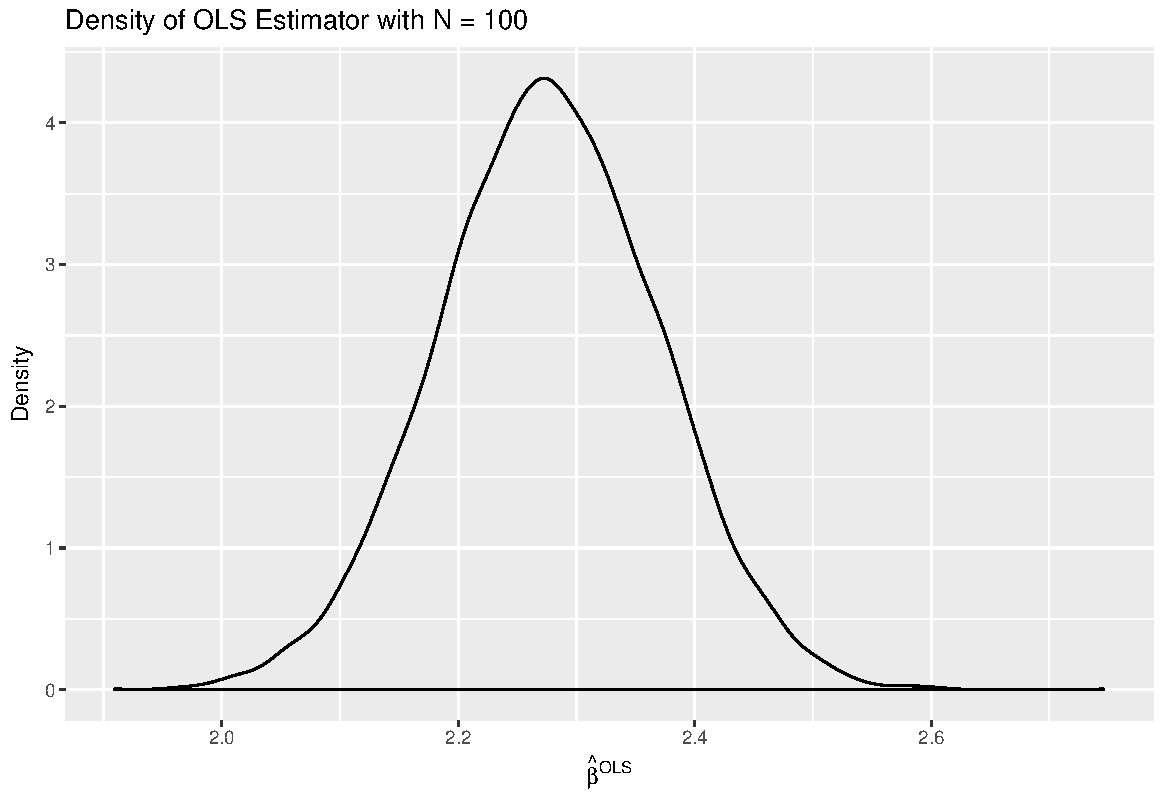
\includegraphics[width=.3\textwidth]{ols_smallN.pdf}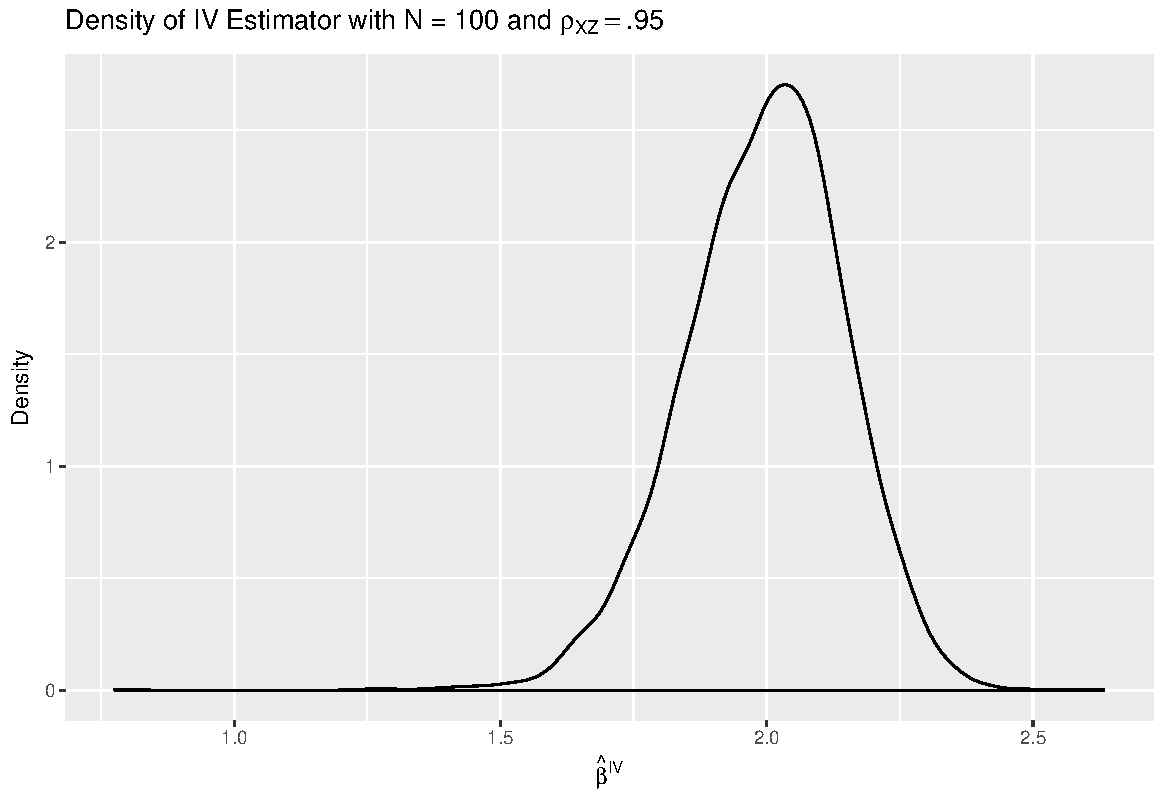
\includegraphics[width=.3\textwidth]{strongIV_smallN.pdf}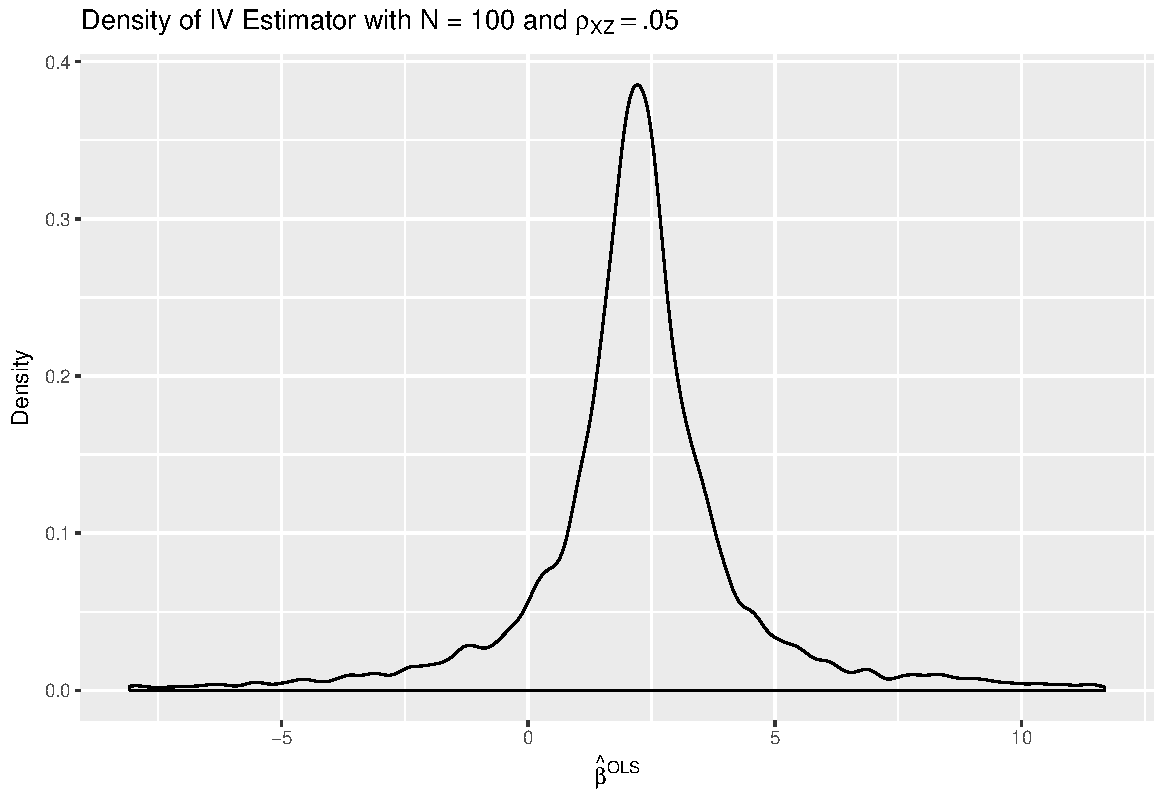
\includegraphics[width=.3\textwidth]{weakIV_smallN.pdf}
\end{figure}

\begin{itemize}{\footnotesize
\item OLS is biased with $\mu=2.27$ and $\sigma^2=.008$
\item Strong IV is unbiased (asymptotically) with $\mu=1.99$ and $\sigma^2 = .024$
\item Weak IV is unbiased (asymptotically) with $\mu=2.05$ but $\symbf{\sigma^2 = 1653.11}$
}
\end{itemize}

\end{frame}



\begin{frame}{The Sampling Distribution of $\hat\beta$}
\begin{align*}
	Y = 1 + 2 X + \varepsilon
\end{align*}

\begin{figure}
\centering \caption{\small Distribution of $\hat\beta$ for OLS, weak IV, strong IV with $N=10000$}
	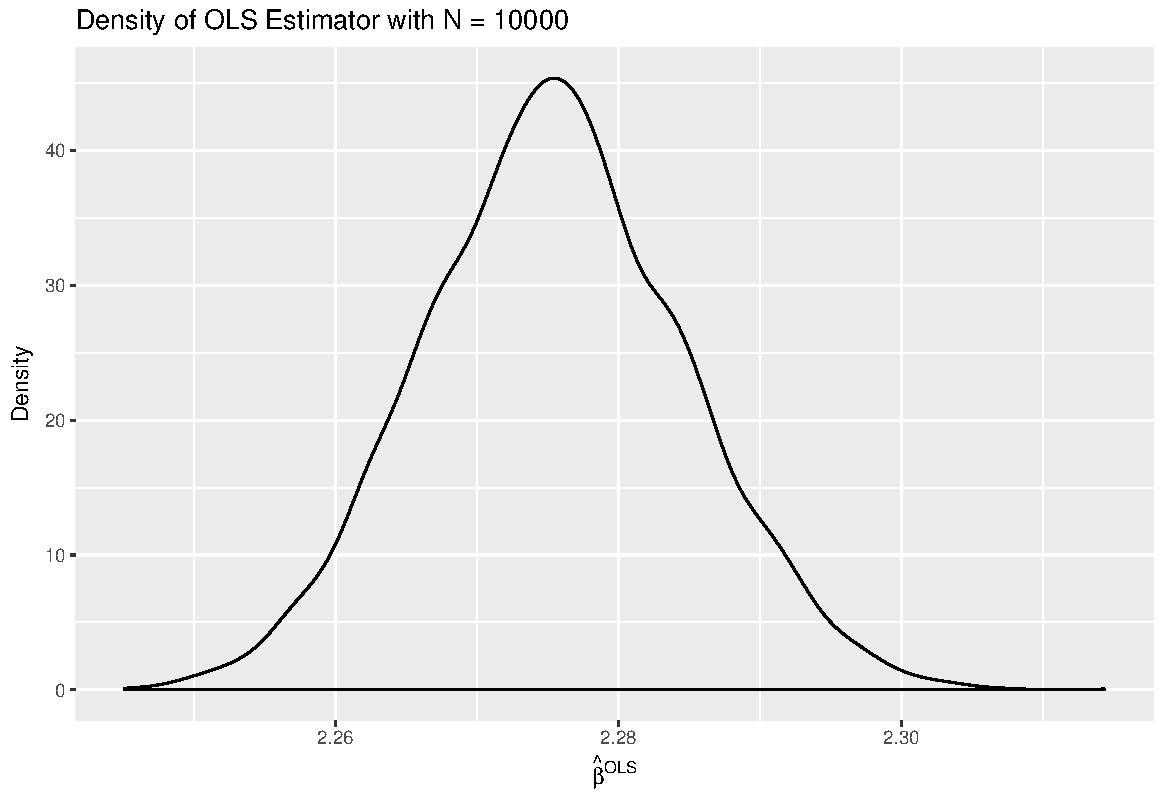
\includegraphics[width=.3\textwidth]{ols_largeN.pdf}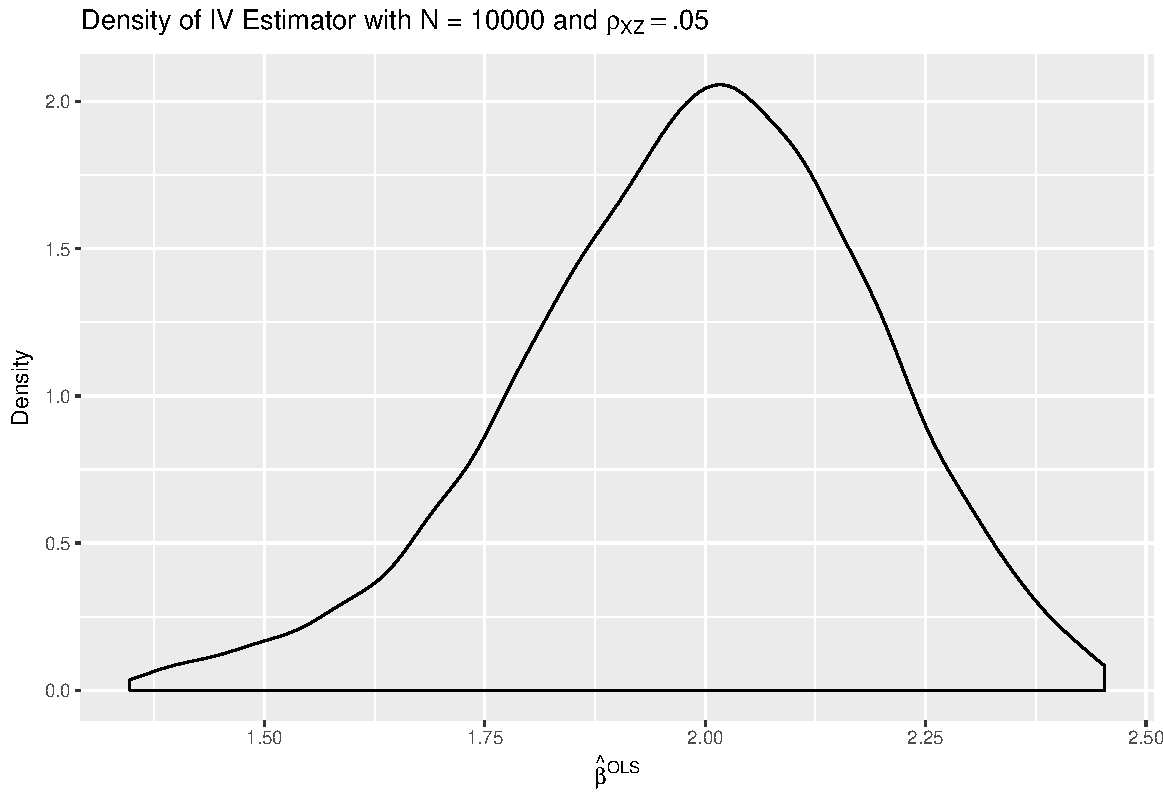
\includegraphics[width=.3\textwidth]{weakIV_largeN.pdf}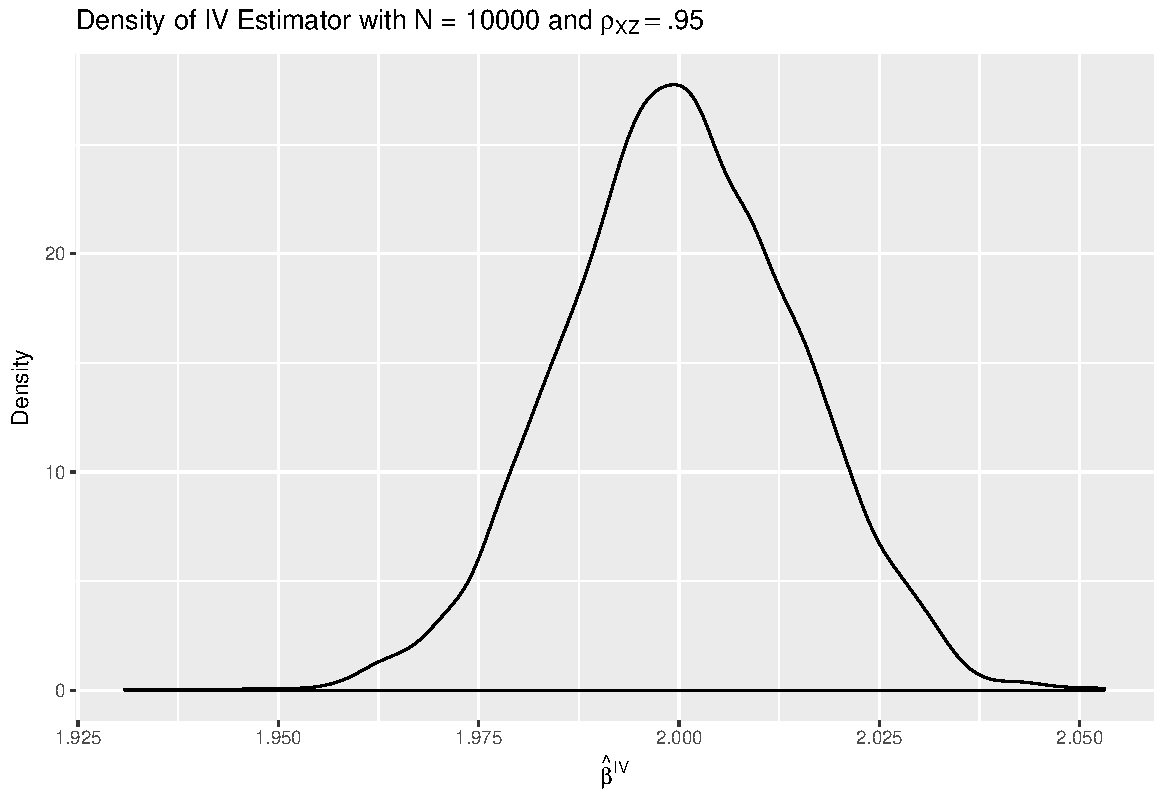
\includegraphics[width=.3\textwidth]{strongIV_largeN.pdf}
\end{figure}

\begin{itemize}{\footnotesize
\item OLS remains biased with $\mu=2.28$ and $\sigma^2=.000085$
\item Strong IV is consistent with $\mu=1.99$ and $\sigma^2 =.00021$
\item Weak IV is consistent with $\mu=2.05$ and even with $N=10k$, $\sigma^2 = .05$
	\begin{itemize}{\scriptsize
		\item Still over 100x larger variance than strong instruments!
	}
	\end{itemize}
}
\end{itemize}
\end{frame}


\begin{frame}{What is the Danger of the CLT Failing?}

	\begin{itemize}
		\item With weak IV, CLT fails and behaves poorly even if $N$ is large
		\item Remember that for testing we want to reject the null hypothesis incorrectly 5\% of the time
			\begin{itemize}
				\item When the CLT fails, our trusty 1.96 critical value is way off base
				\item Example rejection probabilities for test that $\hat\beta=2$
				\begin{table}[H]
				\centering
				\begin{tabular}{rr}
						{\bf Hypothetical Situation} & $P(|t|>1.96)$ \\
						Weak IV, $N=100$ &  0.3\% \\
						Strong IV, $N=100$ & 4.2\% \\
						Weak IV, $N=10000$ & 3.2\% \\
						Strong IV, $N=10000$ & 5.1\% \\
				\end{tabular}
				\end{table}
				\item Goal should be 5\% but for weak IV with $N$ small, almost never reject; still only 3\% even for $N$ large---this is a bad test!

			\end{itemize}
	\end{itemize}
\end{frame}



\begin{frame}[fragile]\frametitle{Example in \texttt{R}: Checking Angrist \& Evans Validity}
\begin{lstlisting}[frame=single]  % Start your code-block
		gross
 # First Stage Test in Angrist & Evans
flm1 = feols(morekids ~ samesex + black + hispan, data=babyData)
lh1 = linearHypothesis(flm1,"samesex = 0", test="F")

# First Stage Test in AE w/ Multiple Instruments
flm2 = feols(morekids ~ boyBoy + girlGirl + black + hispan, data=babyData)
lh2 = linearHypothesis(flm2,c("BoyBoy","GirlGirl"), test="F")
\end{lstlisting}

\vspace{3mm}
	Results:
\begin{itemize}
	\item With ``Same Sex": $F = 25.874$
	\item With ``BoyBoy" and ``GirlGirl": $F = 12.94$
\end{itemize}
\end{frame}




\begin{frame}{Checking The IV Assumptions II}

\begin{itemize}
\item The two major assumptions:
\begin{enumerate}
	\item Relevance: $Cov(X,Z)\ne 0$, or that $\E\left[{\bf z}_i {\bf x}_i' \right]$ has full rank

	\item Exogeneity: All instruments must be uncorrelated with $\varepsilon$
\end{enumerate}
\smallskip
	\item Now, let's talk about the exogeneity assumption.
	\item With one IV, it's impossible to test exogeneity, hence
	the need to evaluate exogeneity by thinking about whether
	some unobserved variables might be correlated with the instrument.
	\item Two popular tests:
	\begin{enumerate}
		\item Hausman-Wu Test: Are $\widehat{\beta}_{IV}$ and $\widehat{\beta}_{OLS}$ the same?
		\item Sargan $J$ Test: If we leave out $z_{i}^{*}$ from our regression does $\E[(Y_i -  X_i \widehat{\beta}_{2SLS})\, z_i^*]=0$?
	\end{enumerate}
	\item These have fallen out of favor because they don't make sense if we have \alert{heterogeneous treatment effects} (ie: $\beta_i$).
	\item Why? \alert{different instruments} identify \alert{different complier} groups.
	% \item With extra instruments, we can test the IVs against each other.
	% Similarly, one IV allows us to test the validity of OLS.
	% \item In all cases, the most we can do is test one exogeneity assumption
	% against another, we can never test the validity of an exogeneity assumption on its own.
\end{itemize}
\end{frame}



\begin{frame}{Overidentification}
\begin{itemize}
	\item When the number of regressors equals the number of instruments,
	the model is {\bf just identified}. When there are
	more instruments than regressors, the model is {\bf overidentified}.

	\medskip
	\item For a just identified model, the 2SLS estimator simplifies to\[
	\mathbf{b}_{IV}=\left(\mathbf{Z}'\mathbf{X}\right)^{-1}\mathbf{Z}'\mathbf{y},
	\]
	which is often called simply the {\bf IV estimator}.

	\medskip
%	\item (Derivation on board)
\end{itemize}
\end{frame}

\begin{frame}{A Note on Moments}
\begin{itemize}
	\item Recall the property of the OLS estimator:
\begin{align*}
	\mathbf{X}'\mathbf{e}_{OLS}&=\mathbf{0}, \text{ with }
	\mathbf{e}_{OLS}=\left(\mathbf{y}-\mathbf{X}\mathbf{b}_{OLS}\right)
\end{align*}
	\item Similarly, for the IV estimator,
\begin{align*}
	\mathbf{X}'\mathbf{e}_{IV}&=\mathbf{0}, \text{ with }
	\mathbf{e}_{IV}=\left(\mathbf{y}-\mathbf{X}\mathbf{b}_{IV}\right)
\end{align*}
\item A consequence of this is that we can't
	test the assumption that the instrument(s) and
	error terms are uncorrelated by looking at the
	correlation between the instrument(s) and residuals.

	\smallskip
	\item Similarly, the residuals from OLS don't allow
	us to test whether the error terms are correlated with the
	regressors.
	\item Stories about an IV being \alert{excluded} are \alert{just a story}.
\end{itemize}
\end{frame}



\begin{frame}{Tests of Exogeneity?}
One possibility is the \alert{Durbin-Wu-Hausman Test} which compares $\Delta = \widehat{\beta}_{OLS} - \widehat{\beta}_{2SLS}$ under the null that $X$ is \alert{exogenous} ($Z$ is assumed exogenous).
\begin{align*}
H_0: & \beta_{OLS}, \beta_{2SLS} \text{ are consistent, }\quad \beta_{OLS} \text{ is efficient }\\
H_1: & \beta_{2SLS} \text{ is consistent, } \beta_{OLS} \text{ is not }.
\end{align*}
This gives a chi-squared test statistic:
\begin{align*}
T = \Delta^T\, (V(\widehat{\beta}_{2SLS}) - V(\widehat{\beta}_{OLS}))^{\dagger}\, \Delta \sim \chi^2_{K}
\end{align*}
This uses the \alert{pseudo inverse} of the variance matrix where $K$ is the rank of that matrix.\\
\medskip
Idea: Reject $H_0$ if $\norm{\Delta} \gg 0$ (2SLS and OLS disagree).
\end{frame}


\begin{frame}{Tests of Exogeneity?}
The other possibility is the \alert{Sargan J-Test} which exploits \textbf{overidentification} (more instruments that endogenous regressors)
\begin{enumerate}
	\item Pick an instrument(s) $z_{i}^* \in \mathbb{R}^{N \times L}$ to drop.
	\item Run 2SLS using remainder except $z_{i}^*$ to get $\widehat{\beta}_{2SLS}^{*}$ with $K$ restrictions.
	\item Evaluate the \alert{moment condition}: $g_n(\widehat{\beta}_{2SLS}^*) = \E[(Y_i - X_i \widehat{\beta}_{2SLS}^{*})\, z_i^*]$.
	\item Construct the quadratic form: $J = g_n(\widehat{\beta}_{2SLS}^*)^T\, W\, g_n(\widehat{\beta}_{2SLS}^*) \sim \Chi^2_{L-K}$ where $L-K$ are the number of extra moments (dimension of $z_i^{*}$).
\end{enumerate}
\end{frame}



\begin{frame}{Software reports all three}

\begin{figure}
\centering
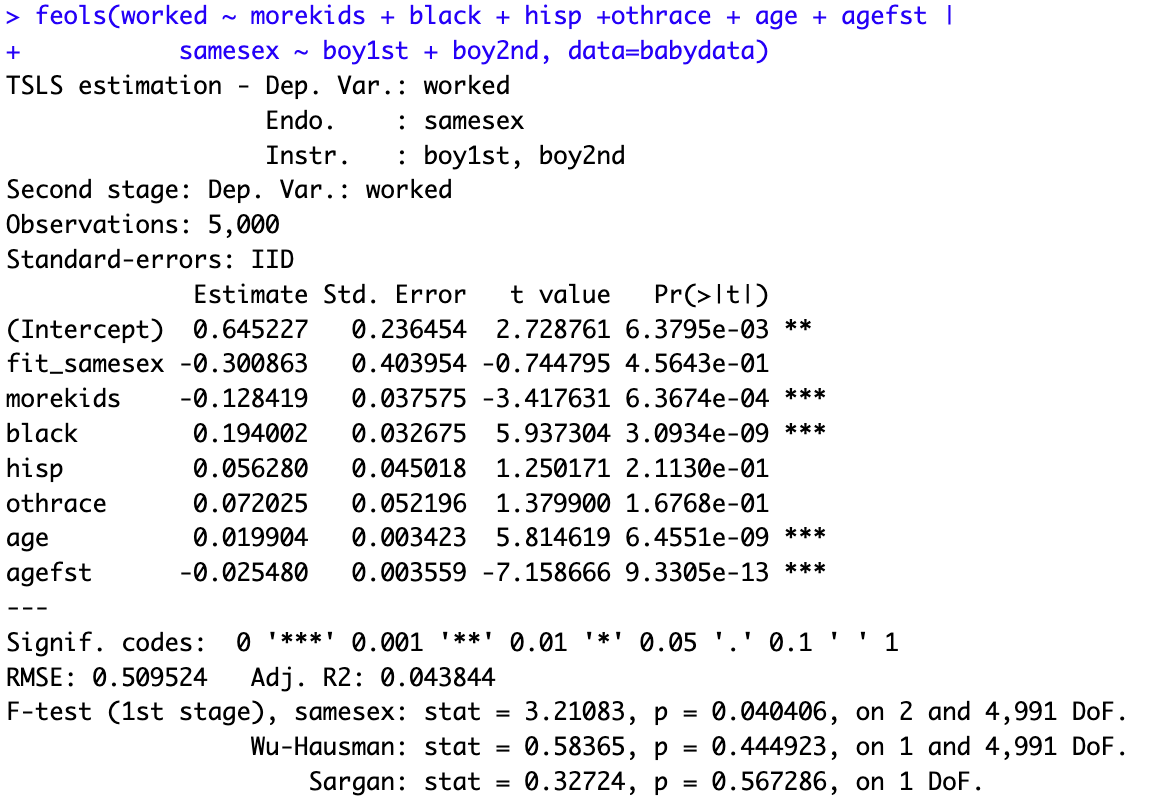
\includegraphics[height=0.9\textheight]{test_statistics}
\end{figure}

\end{frame}



\begin{frame}{Discussion / Practical Tips}
\begin{enumerate}
	\item We really want \alert{strong instruments} that are good predictors of the \alert{endogenous} $X$'s.
	\item Everyone expects us to show the \alert{first-stage F-statistic} telling us whether \alert{excluded instruments} predict endogenous $X$ \alert{beyond the exogenous regressors}.
	\begin{itemize}
		\item With appropriate clustering/standard errors we want to see $F>10$. This is \alert{large enough in practice} but probably \alert{not in theory}!
		\item Ideally we'd have a much stronger $F$-stat but good IV are hard to come by
	\end{itemize}
	\item We can't really test \alert{exclusion} or \alert{exogeneity} of your instruments. 
	\begin{itemize}
		\item This is largely a story that comes from some economic theory or understanding of the world. 
	\item There are tests but they don't show what we really care about
	\begin{itemize}
		\item Wu-Hausman shows us if $\beta_{IV} = \beta_{OLS}$ (not if instruments are valid)
		\item Sargan shows us if different instruments give the same $\widehat{\beta}_{2SLS}$ (which might be because of \alert{heterogeneous treatment effects}).
	\end{itemize}
	\end{itemize}
\end{enumerate}
\end{frame}










\begin{frame}{Weak instruments after 2020: $F > 10$ was never enough}
\begin{itemize}
	\item Staiger--Stock's $F > 10$ keeps the \emph{bias} of 2SLS under $10\%$ of the OLS bias. It says
	nothing about the size of the $t$-test.
	\item Lee, McCrary, Moreira and Porter (2022): with one instrument, the $5\%$ 2SLS $t$-test can reject a
	true null up to $15\%$ of the time at $F \approx 10$. Guaranteeing $5\%$ size with the usual critical
	value needs $F > 104.7$; their \alert{$tF$ procedure} inflates the critical value with the observed $F$ instead.
	\item Simulated, one instrument, $\rho = 0.95$, true $\beta = 0$:
\end{itemize}
\begin{center}
\small
\begin{tabular}{ccc}\toprule
Mean first-stage $F$ & 2SLS $t$-test, actual size & Anderson--Rubin test, actual size \\ \midrule
11 & 0.094 & 0.045 \\
105 & 0.049 & 0.052 \\
\bottomrule\end{tabular}

\end{center}
The $t$-test over-rejects at $F \approx 10$ and is fine at $F \approx 100$; Anderson--Rubin is fine at both.
\end{frame}


\begin{frame}{Anderson--Rubin: inference that does not care how weak the instrument is}
\begin{itemize}
	\item To test $H_0: \beta = \beta_0$, form $y_i - \beta_0 x_i$ and regress it on the instrument. Under $H_0$
	and exclusion, the coefficient is zero \emph{whatever the first stage looks like}: the test never divides by
	the first stage, so weakness cannot distort it.
	\medskip
	\item Invert it: the \alert{AR confidence set} is the set of $\beta_0$ not rejected. With a strong
	instrument it is close to the usual interval; with a weak one it is wide, possibly unbounded, and that
	is the honest answer. (A $95\%$ interval that is always finite cannot be valid under weak instruments
	--- Dufour 1997.)
	\medskip
	\item Just-identified, one endogenous variable: this is a grid search over $\beta_0$ with one regression
	each, a dozen lines of code (workbook).
	\medskip
	\item Practical rule for this course: report the first-stage $F$; if it is below $\approx 100$, also report
	the AR interval. \texttt{ivDiag} and \texttt{ivmodel} in R do it; \texttt{linearmodels} in Python.
\end{itemize}
\end{frame}

\section{Local average treatment effects}

\begin{frame}{When effects differ across people, what does IV estimate?}
\begin{itemize}
	\item Session 6 wrote $y_i = \beta_0 + \beta_1 D_i + \varepsilon_i$ with \emph{one} $\beta_1$. In business data the
	effect of a loan, an app, a refund, a training program differs across customers, and the ones who take it
	up are not a random draw.
	\medskip
	\item Setup (Imbens and Angrist 1994): binary treatment $D_i$, binary instrument $Z_i$. Two sets of potential
	outcomes: \alert{potential treatments} $D_i(1), D_i(0)$ (what $i$ does if $Z_i = 1$ or $0$) and potential
	outcomes $Y_i(1), Y_i(0)$.
	\medskip
	\item Running example: a retailer emails a random half of its customers ($Z_i$) encouraging them to install
	the loyalty app ($D_i$). Outcome: spending next quarter. Some customers would install it anyway; some never
	will; some install it \emph{because} of the email.
	\medskip
	\item Readings: Hansen Ch.~12.29--12.31; Goff Ch.~4; Mixtape Ch.~7.
\end{itemize}
\end{frame}


\begin{frame}{Four types of customer, two of which you cannot see}
\begin{center}
\begin{tabular}{r|cc}
 & $D_i(0) = 0$ & $D_i(0) = 1$ \\
\hline
$D_i(1) = 0$ & \alert{never-taker} & defier \\
$D_i(1) = 1$ & \alert{complier} & \alert{always-taker} \\
\end{tabular}
\end{center}
\begin{itemize}
	\item \alert{Always-takers} install the app with or without the email. \alert{Never-takers} do not install it
	either way. \alert{Compliers} install it only if emailed. \alert{Defiers} install it only if \emph{not} emailed.
	\medskip
	\item We observe $(Z_i, D_i)$, never the pair $(D_i(0), D_i(1))$. A customer with $Z_i = 1, D_i = 1$ is an
	always-taker or a complier; we cannot tell which. That is the whole difficulty.
	\medskip
	\item Three assumptions:
	\begin{enumerate}
		\item \alert{Independence}: $Z_i \perp \big(Y_i(1), Y_i(0), D_i(1), D_i(0)\big)$. The email is randomized.
		\item \alert{Exclusion}: $Z_i$ affects $Y_i$ only through $D_i$. The email itself does not change spending.
		\item \alert{Monotonicity}: $D_i(1) \ge D_i(0)$ for everyone. No defiers.
	\end{enumerate}
\end{itemize}
\end{frame}


\begin{frame}{The LATE theorem in three lines}
\small
Write $D_i = D_i(0) + \big(D_i(1) - D_i(0)\big) Z_i$ and $Y_i = Y_i(0) + \big(Y_i(1) - Y_i(0)\big) D_i$.
\begin{align*}
	\E[Y_i \mid Z_i = 1] - \E[Y_i \mid Z_i = 0]
	&= \E\big[(Y_i(1) - Y_i(0))\,(D_i(1) - D_i(0))\big] && \text{(independence + exclusion)} \\
	&= \E\big[Y_i(1) - Y_i(0) \mid D_i(1) > D_i(0)\big] \cdot \Pr\big(D_i(1) > D_i(0)\big) && \text{(monotonicity: } D_i(1) - D_i(0) \in \{0, 1\}) \\
	\E[D_i \mid Z_i = 1] - \E[D_i \mid Z_i = 0] &= \Pr\big(D_i(1) > D_i(0)\big) && \text{(the first stage is the complier share)}
\end{align*}
Divide:
\begin{align*}
	\beta_{IV} = \frac{\E[Y_i \mid Z_i = 1] - \E[Y_i \mid Z_i = 0]}{\E[D_i \mid Z_i = 1] - \E[D_i \mid Z_i = 0]}
	= \E\big[Y_i(1) - Y_i(0) \mid \text{complier}\big] \equiv \text{LATE}.
\end{align*}
\begin{itemize}
	\item The Wald estimator from Assignment 3, now with a population it belongs to: the compliers.
	\item Always-takers and never-takers drop out of the numerator because $D_i(1) - D_i(0) = 0$ for them:
	the email did not change what they did, so it cannot reveal what the app did for them.
	\item Without monotonicity, defiers enter with a minus sign and the ratio is a difference of two effects.
\end{itemize}
\end{frame}


\begin{frame}{The encouragement design, simulated}
$10{,}000$ customers: $20\%$ always-takers (effect of the app $2.0$, and they spend more anyway), $40\%$
compliers (effect $0.8$), $40\%$ never-takers (effect $0.5$ if they ever installed it). Email to a random half.
\begin{center}
\small
\begin{tabular}{lcl}\toprule
Quantity & Estimate & What it is \\ \midrule
OLS, $y$ on $D$ & 2.72 (0.03) & effect on the treated $+$ selection (always-takers spend more anyway) \\
Reduced form, $y$ on $Z$ & 0.32 (0.04) & intent-to-treat: effect of the \emph{email} \\
First stage, $D$ on $Z$ & 0.39 (0.01) & share of compliers (truth $0.40$) \\
2SLS $=$ Wald ratio & 0.80 (0.09) & LATE: effect for compliers (truth $0.80$) \\
ATE (truth) & 0.91 & average over everyone, including never-takers \\
ATT (truth) & 1.40 & average over app users: always-takers and encouraged compliers \\
Complier mean tenure & 1.99 & Abadie's $\kappa$ estimate (truth 2.01; always-takers 4.00, never-takers 1.00) \\
\bottomrule\end{tabular}

\end{center}
\end{frame}


\begin{frame}{Reading that table}
\begin{itemize}
	\item \alert{OLS} compares app users to non-users; always-takers are heavy spenders regardless, so it is
	off by a factor of three.
	\item \alert{Reduced form} is the effect of the \emph{email}: what the marketing team cares about, and it
	needs no exclusion restriction.
	\item \alert{First stage} is the complier share: $40\%$ of customers can be moved by an email.
	\item \alert{2SLS} recovers the compliers' effect, $0.8$: not the ATE ($0.91$), not the ATT ($1.40$). No
	estimator from this experiment delivers those, because it never moved the other two types.
	\item \alert{Who are the compliers?} Abadie (2003): for any covariate $X$,
	$\E[X \mid \text{complier}] = \big(\E[X D \mid Z = 1] - \E[X D \mid Z = 0]\big)/\big(\E[D \mid Z = 1] - \E[D \mid Z = 0]\big)$,
	the theorem applied to $XD$. The last row recovers the compliers' mean tenure. Describe your compliers.
\end{itemize}
\end{frame}


\begin{frame}{Different instruments, different compliers, different LATEs}
\begin{itemize}
	\item A second valid instrument (a \$5 credit for installing) moves a different set of customers: price-sensitive
	ones rather than email-responsive ones. Its LATE is the effect for \emph{those} compliers.
	\medskip
	\item Two valid instruments can give two different 2SLS estimates, and the overidentification test from
	earlier today can reject with both instruments perfectly valid. The $J$ test assumes one $\beta$.
	\medskip
	\item Which LATE do you want? The one whose compliers match the policy. ``Should we send more emails?'' wants
	the email LATE. ``Should we make the app opt-out?'' wants an effect on today's never-takers, which no
	encouragement design identifies.
	\medskip
	\item The LATE framework is Vytlacil (2002)'s point in reverse: monotonicity is exactly the assumption that
	treatment is chosen by a single index crossing a threshold, $D_i = \mathbb{1}\{v_i \le \pi(Z_i)\}$, which is
	how every selection model in this course has been written.
\end{itemize}
\end{frame}


\begin{frame}{When monotonicity is the assumption to worry about}
\begin{itemize}
	\item \alert{Encouragement that backfires.} A reminder that annoys some customers into uninstalling: defiers.
	\medskip
	\item \alert{Angrist and Evans (1998).} Two same-sex children as an instrument for a third child: parents who
	want two boys become defiers when they get two girls.
	\medskip
	\item \alert{Judges and examiners}, next section: a judge who is strict on drug cases and lenient on
	property cases is lenient for some defendants and strict for others. Monotonicity across judges is the
	live question in that literature.
	\medskip
	\item De Chaisemartin (2017): with ``a few'' defiers, 2SLS still estimates a LATE for a
	subpopulation of compliers, provided compliers outnumber defiers with the same effects. The theorem is
	tolerant, not fragile.
	\medskip
	\item Exclusion failing is the more common problem in practice, and it is not testable. Ask what else the
	instrument could do.
\end{itemize}
\end{frame}


\section{Judge and examiner designs}

\begin{frame}{Random assignment to a decision-maker}
\begin{itemize}
	\item Many treatments are \emph{decided by a person}: a judge sets bail, a loan officer approves credit,
	a claims adjuster pays or denies, a moderator removes a post, a recruiter advances a candidate, a
	customer-service agent grants a refund.
	\medskip
	\item Decision-makers differ in strictness. If cases are assigned to them \alert{at random}, then which
	decision-maker you drew is a random shock to your treatment probability that has nothing to do with you.
	\medskip
	\item Instrument: the assigned decision-maker's \alert{leniency}, measured as their decision rate on
	\emph{other} cases (leave-one-out).
	\medskip
	\item Canonical: Kling (2006, incarceration), Dobbie and Song (2015, bankruptcy), Maestas, Mullen and
	Strand (2013, disability insurance), Dobbie, Goldin and Yang (2018, pretrial detention); in business,
	Dobbie et al.\ (2021, loan officers). Assignment 4 has loan officers; today, refund requests.
\end{itemize}
\end{frame}


\begin{frame}{Running example: refund requests}
\begin{itemize}
	\item $20{,}000$ refund requests routed at random to $50$ customer-service agents. Agent $j$ grants a
	refund if the claim's merit $q_i$ (which the agent sees and we do not) exceeds the agent's personal
	threshold. Agents differ: some grant $20\%$ of requests, some $60\%$.
	\medskip
	\item Outcome: the customer's spending over the next year. Truth:
	\[
		\text{spend}_i = 100 + \tau_i R_i + 30\,q_i + \varepsilon_i, \qquad \tau_i = 20 - 15\,q_i .
	\]
	A refund builds the most goodwill for customers with \emph{weak} claims (they expected to lose); customers
	with strong claims also spend more regardless, since good customers make good claims.
	\medskip
	\item Question for the business: what does granting a refund do to future spending? Naive answer:
	compare spending of refunded and non-refunded customers.
\end{itemize}
\end{frame}


\begin{frame}{The first stage is the whole design}
\begin{center}
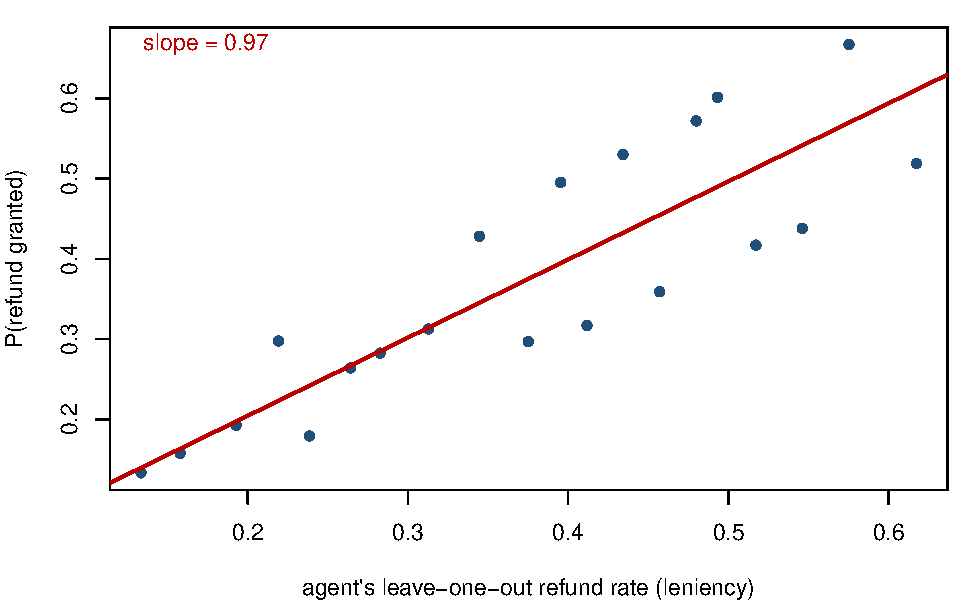
\includegraphics[width=.6\textwidth]{fig_judge_fs.pdf}
\end{center}
\vspace{-.3cm}
{\small Binned: the probability a request is granted against the assigned agent's leave-one-out grant rate. A
slope near one says a request routed to an agent who grants $10$ points more often is $10$ points more likely
to be granted. This picture is the first thing every judge-design paper shows.}
\end{frame}


\begin{frame}{Estimates}
\begin{center}
\small
\begin{tabular}{lccc}\toprule
 & OLS, spend on refund & First stage, refund on leniency & 2SLS \\ \midrule
Coefficient & 47.9 & 0.97 & 15.3 \\
 & (0.6) & (0.004) & (1.7) \\
Truth & ATE $= 19.9$; effect on refunded $= 7.2$ & --- & LATE (marginal claims) $\approx 13.7$ \\
First-stage $F$ & & 1773 &  \\
First stage by claim size & \multicolumn{3}{c}{small 0.86, medium 0.95, large 1.10 (all positive: no sign of defiers)} \\
\bottomrule\end{tabular}

\end{center}
\medskip
\begin{itemize}
	\item OLS is off by a factor of three: refunded customers had better claims and spend more anyway.
	\item 2SLS gives the effect for \alert{marginal} claims: those whose outcome depends on which agent they
	drew. It sits below the ATE because marginal claims have moderate merit and the goodwill effect is
	largest for weak ones. The effect on customers who actually got refunds is smaller still.
\end{itemize}
\end{frame}


\begin{frame}{The three conditions, in this setting}
\begin{itemize}
	\item \alert{Relevance.} Agents differ and the leave-one-out rate predicts the decision (first stage, $F$).
	Leave-one-out keeps the case's own decision, and so its own $q_i$, out of its instrument.
	\item \alert{Exclusion.} The agent affects spending \emph{only} through the decision. Fails if lenient agents
	are also friendlier, faster, or offer store credit. Random routing buys independence, not exclusion.
	\item \alert{Monotonicity.} Any request a strict agent grants, a lenient one would too. Fails if agents rank
	claims differently (generous on shipping, strict on damage, or the reverse): then ``lenient'' is not one dimension.
	\item Testing it (Frandsen, Lefgren and Leslie 2023): first stage positive in every subgroup (claim type,
	size, channel); reduced form monotone in leniency. Our table passes for small, medium, and large claims.
	Necessary, not sufficient.
	\item With many agents, 2SLS on continuous leniency is a weighted average of pairwise LATEs
	(Imbens and Angrist 1994).
\end{itemize}
\end{frame}


\begin{frame}{Practical details that decide whether the design works}
\begin{itemize}
	\item \alert{Is assignment really random?} Rotations, caseload balancing, and specialization break it.
	Regress case characteristics on leniency: nothing should predict it (the experiment's balance test).
	\item \alert{Leniency is estimated.} Few cases per agent makes it noisy and pulls 2SLS toward OLS (many
	weak instruments). Leave-one-out or split-sample leniency; agents with enough cases.
	\item \alert{Cluster by decision-maker.} Cases sharing an agent share the instrument.
	\item \alert{Whose effect?} Marginal cases: right for a policy that moves everyone's threshold (``grant all
	refunds under \$50''), wrong for one that changes what always-granted cases receive.
	\item \alert{Business uses.} Any process with random routing and human discretion is an experiment you
	did not have to run: refunds, credit lines, moderation, fraud holds, rep-offered discounts.
\end{itemize}
\end{frame}


\section{Shift-share designs}

\begin{frame}{Exposure designs}
\begin{itemize}
	\item A national (or global) shock hits local units in proportion to their \alert{pre-existing exposure}:
	\[
		B_m = \sum_{k} s_{mk}\, g_k, \qquad s_{mk} = \text{unit } m\text{'s share in category } k \text{ (predetermined)},\quad g_k = \text{shock to category } k .
	\]
	\medskip
	\item Bartik (1991): local employment growth from national industry growth and local industry mix.
	Autor, Dorn and Hanson (2013): local exposure to Chinese imports. Now everywhere: banks' sector mix
	$\times$ sector credit shocks; retailers' category mix $\times$ national category demand; firms' country
	mix $\times$ tariffs.
	\item Use $B_m$ as an instrument for the local variable it predicts, and estimate that variable's effect
	on a local outcome.
	\item Running example: markets differ in which sectors their banks lend to; national sector credit shocks
	$g_k$ move local credit growth $x_m$; the question is the effect of local credit on firm entry $y_m$. A
	local demand shock $\eta_m$ moves both. Truth: $0.4$.
\end{itemize}
\end{frame}


\begin{frame}{Two ways to believe it}
Why would $B_m$ be uncorrelated with $\eta_m$? Two different arguments, and they need different evidence.
\begin{itemize}
	\item \alert{Shares are exogenous} (Goldsmith-Pinkham, Sorkin and Swift 2020). The instrument is really the
	vector of shares; the shocks weight them. Valid if a market's sector mix is unrelated to its local shocks,
	conditional on controls: a differences-in-differences claim. Evidence: pre-trends and balance on the shares
	that matter (the Rotemberg weights say which).
	\item \alert{Shocks are exogenous} (Borusyak, Hull and Jaravel 2022). Shares can be anything; the national
	shocks $g_k$ are as good as random across many categories. Evidence: many independent shocks, balance at the
	shock level.
	\item Same instrument, same number, different justifications and failure modes. Say which one you rely on.
	Assignment 4 breaks the first and shows the second surviving.
\end{itemize}
\end{frame}


\begin{frame}{Which sectors carry the estimate: Rotemberg weights}
\begin{center}
\small
\begin{tabular}{cccc}\toprule
Sector & shock $g_k$ & Rotemberg weight $\alpha_k$ & just-identified $\hat\beta_k$ \\ \midrule
2 & -1.42 & 0.39 & 0.48 \\
4 & 1.56 & 0.25 & 0.40 \\
6 & 1.24 & 0.15 & 0.17 \\
1 & 1.12 & 0.12 & 0.66 \\
5 & -0.56 & 0.07 & 0.47 \\
3 & 0.18 & 0.00 & 4.39 \\
\midrule 2SLS with $B_m$ & & $\sum_k \alpha_k = 1$ & 0.44 $= \sum_k \alpha_k \hat\beta_k$ \\
\bottomrule\end{tabular}

\end{center}
\vspace{-.2cm}
{\small Goldsmith-Pinkham, Sorkin and Swift: the shift-share 2SLS estimate is a weighted average of the
just-identified estimates you would get using each sector's exposure $s_{mk} g_k$ alone, with weights
$\alpha_k \propto g_k \sum_m s_{mk}\tilde x_m$. Weights can be negative. Here one sector carries most of the
estimate; that is the sector whose share-exogeneity claim needs defending, and its own estimate is what
to compare against the pooled one.}
\end{frame}


\begin{frame}{Inference with few shocks}
\begin{itemize}
	\item $1{,}000$ markets, $6$ sector shocks: the instrument varies through six numbers. Markets sharing a
	dominant sector have nearly the same $B_m$ and, with any sector-level component in the outcome, correlated errors.
	\item Ad\~ao, Koles\'ar and Morales (2019): market-level robust SEs treat $1{,}000$ instrument values as
	independent and can be wildly overconfident.
\end{itemize}
\begin{center}
\small
\begin{tabular}{lcc}\toprule
Design & Nominal size & Actual rejection rate under $H_0$ \\ \midrule
Market-level robust SE, sector shocks in the outcome & 0.05 & 0.73 \\
\bottomrule\end{tabular}

\end{center}
\begin{itemize}
	\item A nominal $5\%$ test rejects a true null most of the time. Fix: standard errors at the \emph{shock}
	level (AKM, or the Borusyak--Hull--Jaravel shock-level regression), which with six shocks means honest, wide
	intervals. The effective sample size is the number of shocks, not units.
\end{itemize}
\end{frame}


\begin{frame}[fragile]{In practice}
\begin{lstlisting}
# LATE: an encouragement design
feols(y ~ 1 | D ~ Z, d)                              # 2SLS = Wald ratio
feols(y ~ Z, d); feols(D ~ Z, d)                    # reduced form, first stage (complier share)
(mean(x[Z==1] * D[Z==1]) - mean(x[Z==0] * D[Z==0])) / (mean(D[Z==1]) - mean(D[Z==0]))   # E[x | complier]
# Judges: leave-one-out leniency, cluster by agent
tot <- tapply(R, agent, sum); n_j <- tapply(R, agent, length); len <- (tot[agent] - R) / (n_j[agent] - 1)
feols(spend ~ 1 | R ~ len, d, cluster = ~agent)
# Shift-share: build B and instrument
B <- as.vector(shares %*% g); feols(y ~ 1 | x ~ B, d, vcov = "hetero")
\end{lstlisting}
\begin{itemize}
	\item Shock-level standard errors: \texttt{ssaggregate} (Borusyak--Hull--Jaravel) or the AKM code; Rotemberg
	weights: \texttt{bartik\_weight} (GPSS). Both are Stata-first; the R ports are on GitHub. The workbook computes
	Rotemberg weights by hand in five lines.
\end{itemize}
\end{frame}


\begin{frame}{Recap}
\begin{itemize}
	\item With heterogeneous effects, IV estimates the \alert{LATE}: the effect for compliers, the people the
	instrument actually moved. Reduced form over first stage; first stage is the complier share; describe the
	compliers with Abadie's trick.
	\medskip
	\item \alert{Judge designs}: random routing to decision-makers of different strictness. Leave-one-out
	leniency, first-stage picture, monotonicity across decision-makers is the assumption to test, cluster by
	decision-maker. Any human-discretion process with random assignment qualifies.
	\medskip
	\item \alert{Shift-share}: exposure to national shocks. Decide whether you believe the shares or the shocks;
	Rotemberg weights say which sectors matter; standard errors belong at the shock level.
	\medskip
	\item \alert{Weak instruments}: $F > 10$ was never enough; report Anderson--Rubin.
\end{itemize}
\end{frame}


\begin{frame}{Workbook time}
\texttt{inclass\_session7.Rmd}:
\begin{enumerate}
	\item Reproduce the encouragement design; change the complier effect and watch which rows of the table move.
	\item Reproduce the refund design; give agents type-specific generosity (lenient on shipping, strict on
	damage) and re-run the subgroup first stages.
	\item Reproduce the shift-share estimate and Rotemberg weights; then drop the top-weight sector and see
	what happens to the estimate and the first-stage $F$.
\end{enumerate}
\end{frame}

\end{document}
